
 
\clearpage{}
\subsection{Example: type constraints}

The following contraint tree is for our $\imap$ example:

\begin{tabbing}
MMMM 	\= MM \= MM \= MM \= MM \= MM \= MM \= MM \= MM \= MM \= MM \= MM \= MM \kill

GROUP $\{ \imap \}$ \\	
	\> $s_0$	\> $ = s_{19}$ \\
	\> $e_0$	\> $\tme e_1 \lor e_{19}$
\\[1ex]
	\> LET \ $\imap$ \\
	\> 		\> $s_{map}$	\> $ = s_1$ 
\\[1ex]
	\>		\> LAMBDA \ \{$f$\} \\
	\>		\> 		\> $s_1$	\> $ = s_f    \lfuna{e_2 \ c_1} s_2$ \\
	\>		\>		\> $c_1$ 	\> $\tme \imap : s_{\imap}$ 
\\[1ex]
	\>		\> 		\> LAMBDA \ \{$xx$\} \\
	\>		\>		\> \> $s_2$		\> $ = s_{xx} \lfuna{e_3 \ c_2} s_3$ 
	\>		\>		\> \> $c_2$		\> $\tme \imap : s_{\imap} \lor \ f : s_f$ 
\\[1ex]
	\>		\>		\> \> $s_3$		\> $ = s_6$ 
	\>		\>		\> \> $e_3$ 		\> $\tme \iReadH s_4 \lor e_6 \lor e_7$  \\
	\>		\>		\> \> $s_3$		\> $ = s_8$  \\	
	\>		\>		\> \> $s_4$		\> $ = s_5$  \\
	\>		\>		\> \> $s_4$		\> $ = s_7$  \\
	\>		\>		\> \> $s_5$		\> $ = \iList \ r_5 \ a_5$ \\
	\>		\>		\> \> $s_7$		\> $ = \iList \ r_7 \ a_7$ \\
	\>		\>		\> \> $s_x$		\> $ = a_7$ \\
	\>		\>		\> \> $s_{xs}$		\> $ = \iList \ r_7 \ a_7$ \\
	\>		\>		\> \> $s_4$		\> $ = \rINST \ s_{xx}$  \\
	\>		\>		\> \> LAMBDA \ $\emptyset$	\\
	\>		\>		\> \> \> $s_6$		\> $ = \rINST \ s_{\iNil}$ 
\\[1ex]
	\>		\>		\> \> LAMBDA \ $\{ x, \ xs \}$					\\
	\>		\>		\> \> \> $s_9$		\> $ = s_{14} \lfuna{e_{8a} \ c_8} s_8$ 
	\> 		\> 		\> \> \> $e_8$		\> $\tme e_9 \lor e_{14} \lor e_{8a}$ 
\\
	\>		\>		\> \> \> $s_{10}$	\> $ = s_{11} \lfuna{e_{9a} \ c_9} s_9$ 
	\>		\>		\> \> \> $e_9$		\> $\tme e_{10} \lor e_{11} \lor e_{9a}$ 
\\[1ex]
	\>		\>		\> \> \> $s_{10}$	\> $= \rINST \ s_{\iCons}$  
\\[1ex]
	\>		\>		\> \> \> $s_{12}$ 	\> $= s_{13} \lfuna{e_{11a} \ c_{11}} s_{11}$ 
	\>		\>		\> \> \> $e_{11}$ 	\> $\tme e_{12} \lor e_{13} \lor e_{11a}$  
\\[1ex]
	\>		\>		\> \> \> $s_{12}$	\> $= \rINST \ s_f$ \\
	\>		\>		\> \> \> $s_{13}$	\> $= \rINST \ s_x$ \\
	\>		\>		\> \> \> $s_{15}$	\> $= s_{18} \lfuna{e_{14a} \ c_{14}} s_{14}$ 
	\>		\>		\> \> \> $e_{14}$	\> $\tme e_{15} \lor e_{18} \lor e_{14a}$ 
\\[1ex]
	\>		\>		\> \> \> $s_{16}$	\> $= s_{17} \lfuna{e_{15a} \ c_{15}} s_{15}$ 
	\>		\>		\> \> \> $e_{15}$	\> $\tme e_{16} \lor e_{17} \lor e_{15a}$ 
\\[1ex]
	\>		\>		\> \> \> $s_{16}$	\> $= \rINST \ s_{map}$ \\
	\>		\>		\> \> \> $s_{17}$	\> $= \rINST \ s_{f}$ \\
	\>		\>		\> \> \> $s_{18}$	\> $= \rINST \ s_{xs}$
\\[1ex]
	\> $s_{20}$	\> $= s_{23} \lfuna{e_{19a} \ c_{19}} s_{19}$ \> \> \>
	\> $e_{19}$	\> $= e_{20} \lor e_{23} \lor e_{19a}$ 
\\[1ex]
	\> $s_{21}$	\> $= s_{22} \lfuna{e_{20a} \ c_{20}} s_{20}$ \> \> \>
	\> $e_{20}$	\> $= e_{21} \lor e_{22} \lor e_{20a}$
\\[1ex]
	\> $s_{21}$	\> $= \trm{INST} \ s_{\imap}$ \\
	\> $s_{22}$	\> $= \trm{INST} \ s_{\idouble}$ \\
	\> $s_{23}$	\> $= \trm{INST} \ s_{\ifoo}$ 
\end{tabbing}

\clearpage{}

The constraint tree echos the abstract syntax tree. We have retained the overall structure of the program, while dispensing with details such as distinction between case alternatives and lambda abstractions, and the order of function applications. Once constraints have been extracted, the inference algorithm can ignore the source program entirely. In our real implementation we use a source language that has more sugar than the one presented here, but the constraint language is the same.

Before discussing how to actually solve the constraints, note that there are several degrees of freedom in their ordering. Within a particular LAMBDA, LET or GROUP block it is always safe to move $=$ or $\tme$ constraints earlier in the block. It is also safe to move these constraints up and earlier in the tree, such as moving $s_{\imap} = s_1$ so it appears directly after $e_0 \tme e_1 \lor e_{19}$. Moving these constraints higher up in the tree means they will be considered earlier, and such modifications will not degrade the final constraint solution. It is also safe to change the order of LAMBDA or LET blocks at the same level. This simply corresponds to changing the order of let-bindings or case-alternatives in the original program. On the other hand, in general it is \emph{not} safe to move INST constraints as they control the order in which types are instantiated.

Although we will discuss recursion more fully in \S\ref{inference:ordering}, the structure of the constraints reveals that $\imap$ is recursively defined. This is evident from the fact that $s_{16} = \trm{INST} \ s_{\imap}$, present in the lower quarter of the list, appears inside the LET $\imap$ block. This constraint corresponds to a recursive use of $\imap$. This is in contrast to $s_{21} = \rINST \ s_{\imap}$ which appears outside the block and corresponds to a non-recursive use. Without polymorphic recursion, all recursive uses of let-bound variables should be at identical types, so we will change $s_{16} = \trm{INST} \ s_{\imap}$ to $s_{16} = s_{\imap}$.

From the structure of tree we see that the INST constraints for $s_4$, $s_{12}$, $s_{13}$, $s_{17}$ and $s_{18}$ all correspond to uses of lambda or pattern bound variables. This is clear because they appear inside a LAMBDA block corresponding to the variable they instantiate. For this example we will also simplify these constraints by identifying the variables on the left and right, giving: $s_4 = s_{\ixx}$, $s_{12} = s_f$, $s_{13} = s_x$ and so on.

We will assume that the types of $\iNil$ and $\iCons$ are known. This allows us to replace the constraints for $s_6$ and $s_{10}$ with fresh instantiations of their type schemes. Although the type of $\iCons$ includes a closure term, we store the closure constraint in the graph instead of directly in its type. The form of our reduction rules require that all constraints involve a single constructor only.

\qq\qq
\begin{tabular}{ll}
$s_6$ 		& $= List \ r_6 \ a_6$ \\
$s_{10}$	& $= a_{10} \lfuna{\bot \ \bot} s_{10a}$ \\
$s_{10a}$	& $= s_{10b} \lfuna{\bot \ c_{10}} s_{10c}$ \\
$s_{10b}$	& $= List \ r_{10} \ a_{10}$ \\
$s_{10c}$	& $= List \ r_{10} \ a_{10}$ \\
$c_{10}$	& $= x : a_{10}$
\end{tabular}

\subsection{Constraint sets and equivalence classes}
\label{Inference:Constraints:sets-and-equiv-classes}

Now we can start building the type graph. In the graph our constraints are organised into a set of \emph{equivalence classes}. Each equivalence class contains a set of types that must be equal, or constrained by an inequality. Equivalence classes can be in one of three forms, depending on the kind of the types contained. Value equivalence classes have the form $\kappa n \sim \ov{s} = \ov{\tau}$, where $\kappa$ is the kind of the class, $n$ is a unique integer identifying it, $\ov{s}$ is a list of type variables, and $\ov{\tau}$ is a set of non-variable types. The intention is for the variables on the left of the $=$ to be identified with the types on the right. Effect and closure classes use $\tme$ instead of $=$, so we write them as $\kappa n \sim \ov{a} \tme \ov{\tau}$. As there are no constructors of region kind, we write region equivalence classes as $\kappa n \sim \ov{s}$. 

For example, when we construct an equivalence class from the following constraint set:
\begin{tabbing}
	MMMM	\= MM	\= M \= MMMMMMM \= M \= MMMMMMMMM \= MM \kill
	\>	$\{$	\> $s_1$	\> $= s_f \lfuna{e_2 \ c_1} s_2$, 
			\> $s_{16}$	\> $= s_{17} \lfuna{e_{15a} \ c_{15}} s_{15}$,
	\\
	\>		\> $s_{16}$	\> $= s_{map}$,
			\> $s_{1}$	\> $= s_{map}$
			\> $\}$
\end{tabbing}
we get:

\code{
	*0 &	$\sim \quad s_{map}$, & $s_1$,		& $s_{16}$	& \quad	$=$	
			& $s_f \lfuna{e_2 \ c_1} s_2$,
			& $s_{17} \lfuna{e_{15a} \ c_{15}} s_{15}$
}


This class has the kind of value types and is identified as class 0. The variable that comes first in the list is the \emph{canonical name} for the class.  The canonical name is the variable that we choose to represent the class, and when doing inference by hand we choose the name that is most ``interesting''. In this case we have chosen $s_{map}$ as more interesting than $s_1$ or $s_{16}$, but this choice will not affect the substance of our constraint solution. When a new type variable is added to an equivalence class we substitute the canonical name for occurrences of this variable in the graph. The two types on the right of the = come from the $s_1 = s_f \lfuna{e_2 \ c_1} s_2$ and $s_{16} = s_{17} \lfuna{e_{15a} \ c_{15}} s_{15}$ constraints.

We refer to the set of equivalence classes as ``the type graph'' to distinguish it from the set of constraints which it is built from. Constraint sets and equivalence classes express similar information, but are not completely interconvertible. An equivalence class contains variables and type constructors from the constraint set, but no information about how to match them up. For example, from the equivalence class above we cannot tell if the original constraint set contained $s_1 = s_{map}$, $s_1 = s_{16}$, or both. An equivalence class records a set of types that are all equal, but not exactly why. The fact that this information is is lost will not matter until we discuss error reporting in \S\ref{inference:errors}. Until then we will use equivalence classes, as this notation is more compact. 

\subsection{Example: type graph}

Continuing on with our $\imap$ example, we will add all constraints up to the end of the LET $\imap$ block to the type graph. The result is shown on the next page. Note that we have elided classes that contain only a single variable, such as for $r_4$ and $e_1$.

The form of the type graph already suggests how we should proceed from here. Note that the class for $s_{\imap}$ (*1) contains two type constructors $s_{f} \lfuna{e_{15a} \ c_{15}} s_{15}$ and $s_f \lfuna{e_2 \ c_1} s_2$. These represent the use and definition of $\imap$ respectively. Unifying these two types implies that the  classes for $s_{15}$ (*13) and $s_{2}$ (*5) should be merged. This induces the unification of $s_{xx}$ and $s_{xs}$, which implies that the input list must have the same type as its tail, as expected.
\begin{center}
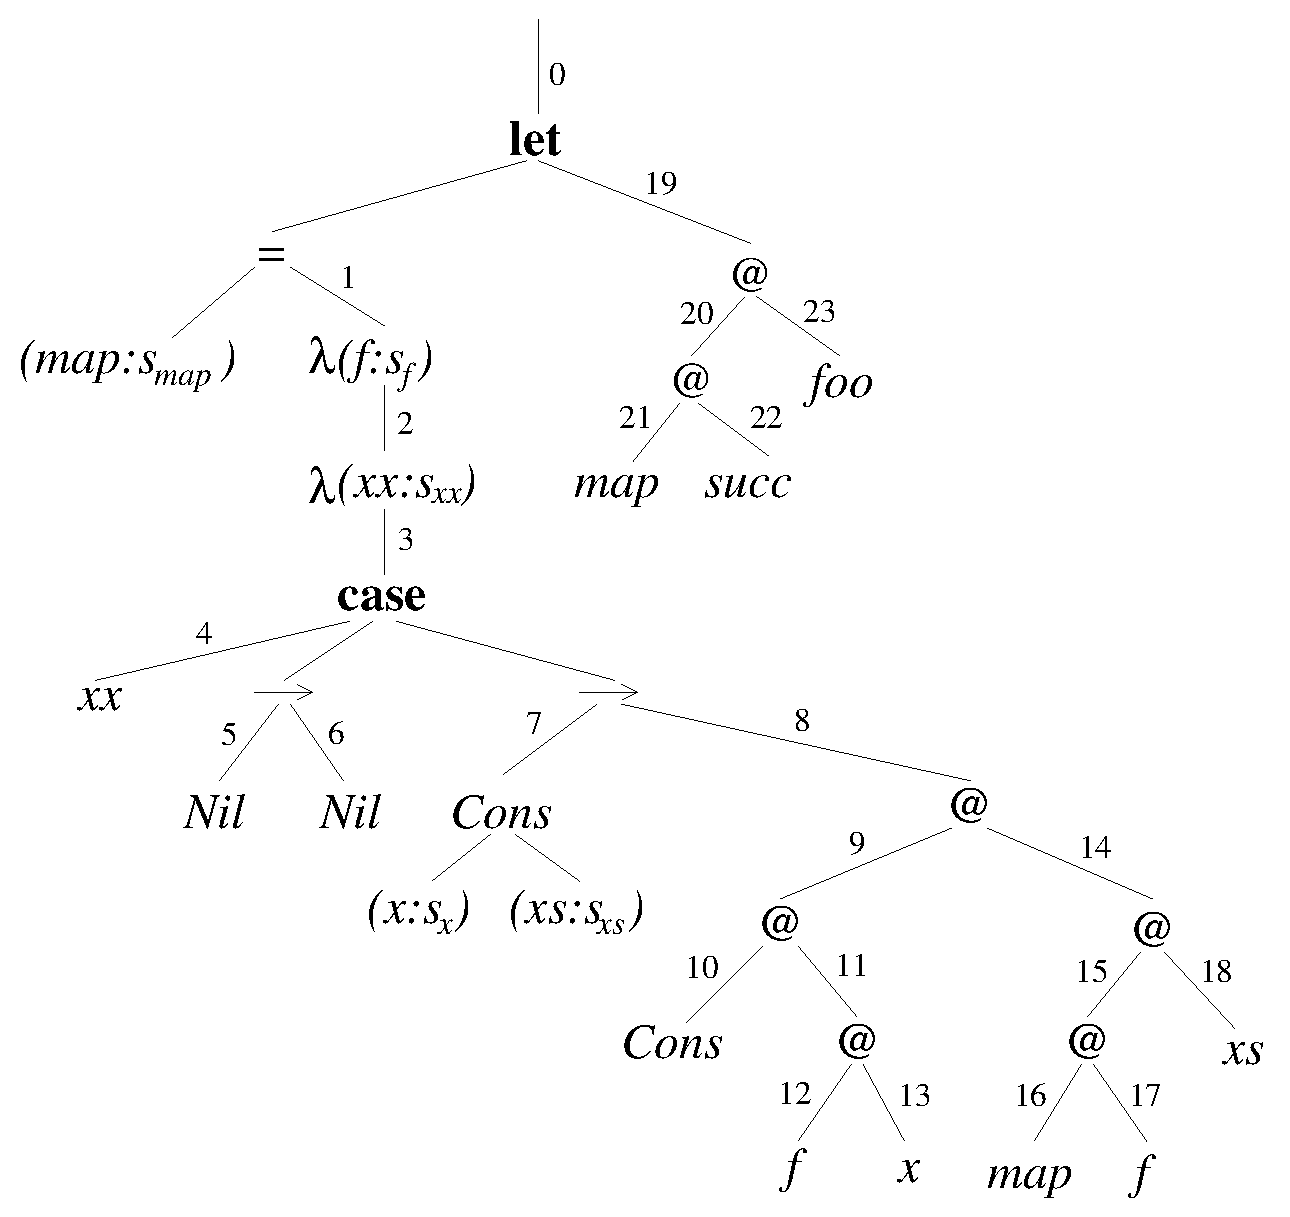
\includegraphics[scale=0.4]{3-Inference/fig/constraints/example-map}
\end{center}

\bigskip
\begin{tabular}{llllllll}
*0 	& $\sim \quad s_0$,	& $s_{19}$	&	& \quad $=$	& $\emptyset$ 
	\\[0.5ex]
*1 	& $\sim \quad s_{map}$, & $s_1, \ s_{16}$ &	& \quad	$=$	& $s_{f} \lfuna{e_{15a} \ c_{15}} s_{15}$, 
									& $s_f \lfuna{e_2 \ c_1} s_2$
	\\[0.5ex]
*2	& $\sim \quad s_f$,	& $s_{17}, \ s_{12}$ &	& \quad $=$	& $s_x \lfuna{e_{11a} \ c_{11}} s_{11}$
	\\[0.5ex]
*3	& $\sim \quad s_x$,	& $s_{13}, \ a_7$ &	& \quad $=$	& $\emptyset$
	\\[0.5ex]
*4	& $\sim \quad s_{xs}$,	& $s_{18}$	&	& \quad $=$	& $\iList \ r_7 \ a_7$
	\\[0.5ex]
*5	& $\sim \quad s_2$	& 		&	& \quad $=$	& $s_{xx} \lfuna{e_3 \ c_2} s_3$
	\\[0.5ex]
*6	& $\sim \quad s_3$,	& $s_6, \ s_8$	&	& \quad $=$	& $\iList \ r_6 \ a_6$
	\\[0.5ex]
*7	& $\sim \quad s_{xx}$,	& $s_4, \ s_5, \ s_7$ &	& \quad $=$	& $\iList \ r_5 \ a_5$,
									& $\iList \ r_7 \ a_7$
	\\[0.5ex]
*8	& $\sim \quad s_9$	&		&	& \quad $=$	& $s_{14} \lfuna{e_{8a} \ c_{3}} s_3$
	\\[0.5ex]
*9	& $\sim \quad s_{10}$	&		&	& \quad $=$	& $s_{11} \lfuna{e_{9a} \ c_{9}} s_9$,
									& $a_{10} \lfuna{\bot \ \bot} s_{10a}$
	\\[0.5ex]
*10	& $\sim \quad s_{10a}$	&		&	& \quad $=$	
							& \mc{2}{$s_{10b} \lfuna{\bot \ c_{10}} s_{10c}$}
	\\[0.5ex]
*11	& $\sim \quad s_{10b}$	&		&	& \quad $=$	& $List \ r_{10} \ a_{10}$
	\\[0.5ex]
*12	& $\sim \quad s_{10c}$	&		&	& \quad $=$	& $List \ r_{10} \ a_{10}$
	\\[0.5ex]
*13	& $\sim \quad s_{15}$	&		&	& \quad $=$	& $s_{xs} \lfuna{e_{14a} \ c_{14}} s_{14}$
	\\[0.5ex]
\ !0	& $\sim \quad e_0$	&		&	& \quad $\tme$	& $e_1 \lor e_{19}$
	\\[0.5ex]
\ !1	& $\sim \quad e_3$	&		&	& \quad $\tme$	& $\iReadH \ s_{\ixx} \lor e_6 \lor e_8$
	\\[0.5ex]
\ !2	& $\sim \quad e_8$	&		&	& \quad $\tme$	& $e_9 \lor e_{14} \lor e_{8a}$
	\\[0.5ex]
\ !3	& $\sim \quad e_9$	&		&	& \quad $\tme$	& $e_{10} \lor e_{11} \lor e_{9a}$
	\\[0.5ex]
\ !4	& $\sim \quad e_{11}$	&		&	& \quad $\tme$	& $e_{12} \lor e_{13} \lor e_{11a}$
	\\[0.5ex]
\ !5	& $\sim \quad e_{14}$	&		&	& \quad $\tme$	& $e_{15} \lor e_{18} \lor e_{14a}$
	\\[0.5ex]
\ !6	& $\sim \quad e_{15}$	&		&	& \quad $\tme$	& $e_{16} \lor e_{17} \lor e_{15a}$
	\\[1ex]
\$1	& $\sim \quad c_1$	&		&	& \quad $\tme$	& $\imap : s_{\imap}$
	\\[0.5ex]
\$2	& $\sim \quad c_2$	&		&	& \quad $\tme$	& $\imap : s_{\imap} \lor f : s_f$
	\\[0.5ex]
\$3	& $\sim \quad c_{10}$	&		&	& \quad $\tme$	& $x : a_{10}$
\end{tabular}

